\chapter{Design of integrated amplifier}

The only way to improve the performance of the spectrometric chain is to integrate the preamplifier, amplifier and a shaper into a small PCB since the ORTEC setup does not allows any upgrades. That includes shortening the signal routes, reducing parasitic capacitances at preamplifier input and improving the shielding. The various prototypes were designed as double-sided PCBs and manufactured by using the milling machine. The PCB consisting mainly of surface mount deposition (SMD) parts was then assembled by manual soldering.

\section{Electronic schematic and layout}
The main parts of integrated amplifier are: photodiode input connector, preamplifier, second stage amplifier, shaper module, output buffer optimized for 50\nobreakspace$\Omega$ transmission line, bipolar voltage supply for modules and bias voltage supply for photodiode. To surround the sensitive parts with sufficient shielding, the PCB is placed into aluminium box with window drilled for photodiode (figures \ref{PCBbox} and \ref{PCBphyss}). The full schematic of the integrated amplifier can be seen in the figure \ref{schematic} and the real layout for PCB can be seen in the figures \ref{layout top} and \ref{layout bottom}.



\begin{figure}[H]
 \centering
 \includegraphics[scale=0.1, angle = 0]{./pictures/SemiInCrateInside.png}
 \caption{Fully assembled integrated amplifier PCB with attached Cremat modules inside the shielding box.}
 \label{PCBbox}
 
\end{figure}


\begin{figure}[H]
 \centering
 \includegraphics[scale=0.1, angle = 0]{./pictures/SemiInCrate.png}
 \caption{PCB in aluminium box with attached peltier coolers.}
 \label{PCBphyss}
 
\end{figure}



\newpage

\begin{figure}[H]
 \centering
 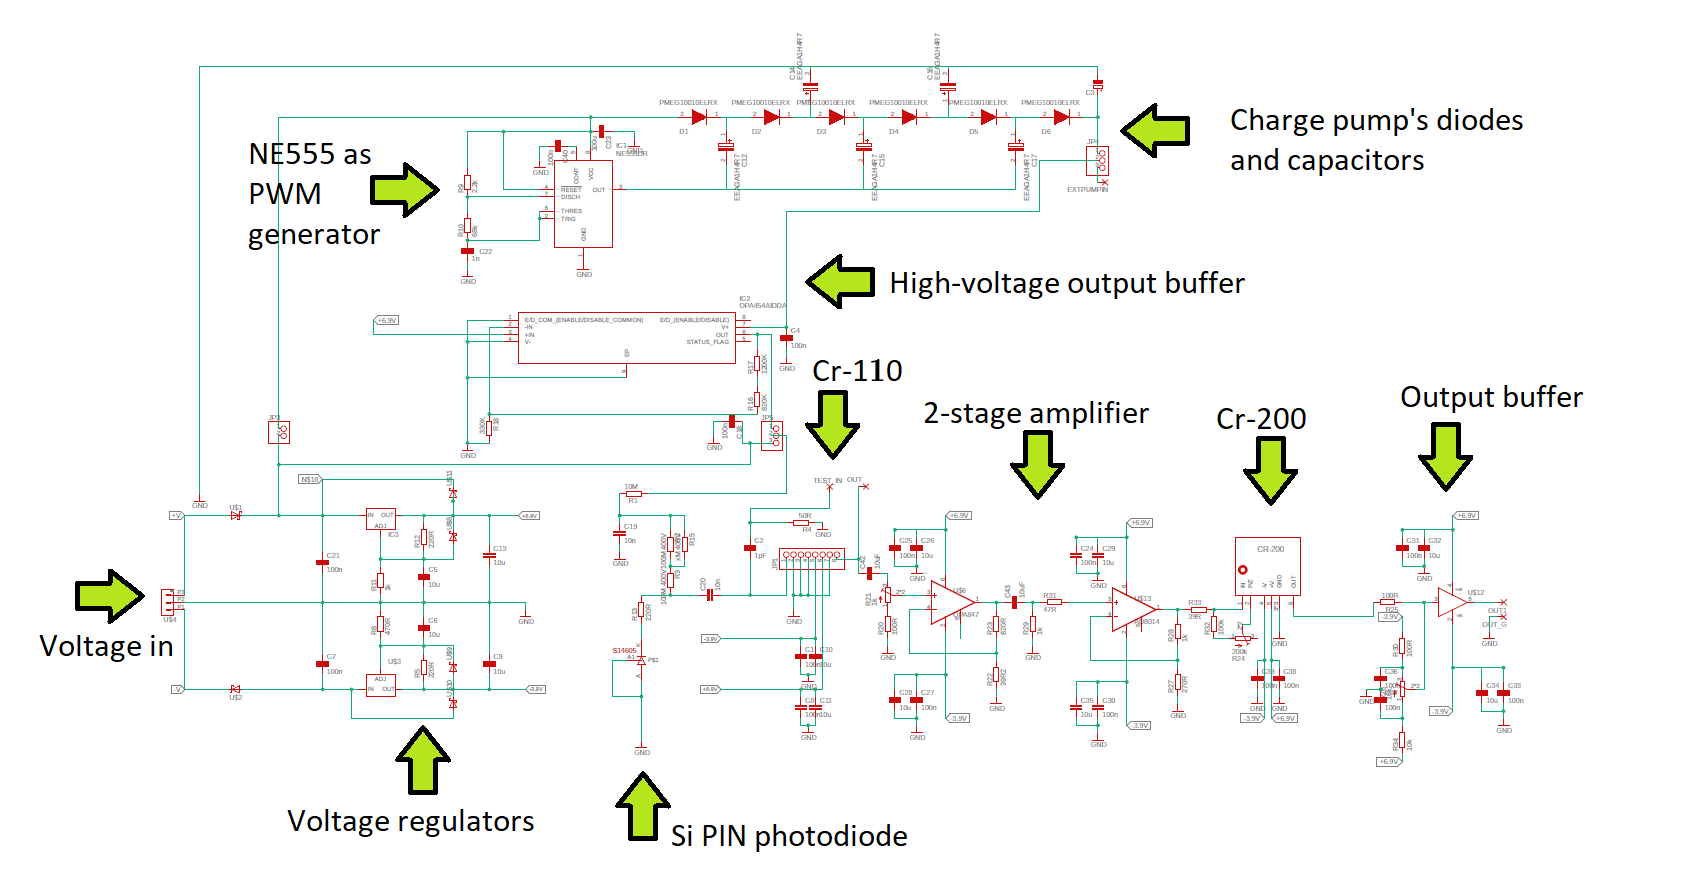
\includegraphics[scale=0.5, angle = 90]{./pictures/schemaPopis.png}
 \caption{Schematic of spectrometric chain PCB designed in EAGLE \cite{eagle}. Full schematic can be found in attachments.}
 \label{schematic}
 
\end{figure}

\newpage

\begin{figure}[H]
 \centering
 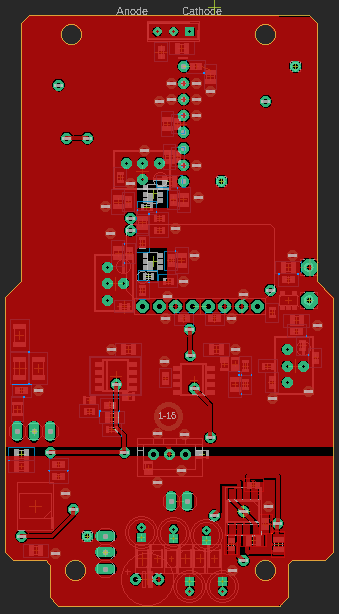
\includegraphics[scale=0.8, angle = 90]{./pictures/S14topLay.png}
 \caption{Layout of spectrometric chain PCB designed in EAGLE \cite{eagle}, top side layer.}
 \label{layout top}
 
\end{figure}

\begin{figure}[H]
 \centering
 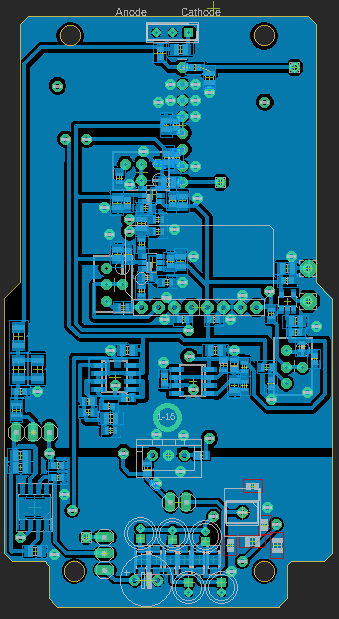
\includegraphics[scale=0.8, angle = 90]{./pictures/S14bottomLay.png}
 \caption{Layout of spectrometric chain PCB designed in EAGLE \cite{eagle}, bottom side layer.}
 \label{layout bottom}
 
\end{figure}
\newpage





\section{Grounding and Shielding}
To allow all the currents to have their return path with a sufficient conductivity, the main GND signal has to be spilled all around the circuit board. Even a small resistances in these paths may cause disturbing voltage dropouts. Currents from non-signal parts such as charge pump should have their return path different from the path of signal parts, and thus the spilled GND has to be cut to two separate parts (signal and bias supply) connected together only at input voltage connector. This kind of layout is reffered as a star ground structure \cite{star}.

\par
The shielding box has to be connected to GND in specific place to prevent the induced currents from shielding to flow over the signal ground of the detector. The best place to connect the shielding box with GND is near the power supply connector.


\section{Photodiode input and preamplifier}
The photodiode is situated inside the box, and the cathode is connected to bias voltage and to preamplifier (CR-110) by capacitive coupling (10 nF capacitor). CR-110 application note also mentions an optional 220 $\Omega$ resistor connected before coupling capacitor to prevent CR-110 breakdown by large current spikes. Our experiences show that this resistor should not be omitted. The signal route from photodiode to preamplifier input has to be as short as possible. 

\section{Amplification and shaping}
The preamplifier output is routed over capacitive coupling (to eliminate unwanted offset) and over potentiometer divider (to adjust signal amplitude) to the amplification stages. First amplification is achieved by two non-inverting amplifiers with OPA847 opamps. Each stage has the amplification of 32$\times$ (or less, this is different for every of our prototypes). Additional amplification 10$\times$ is done by shaper module CR-200. The OPA847 opamp datasheet \cite{OPA847} describes that these fast opamps are prone to unwanted oscillations, and therefore the GND around the opamp must be removed from both sides of the PCB. The output of shaper module is routed directly to output buffer opamp MAX4201, which is connected to the output SMA connector mounted onto the aluminium box.


\section{Voltage supply}
The regulation of power supply (usually +15 V and -15 V) is done by LM317 and LM337 regulators, which convert input supply voltages into +7 V and -4 V. The output voltage of regulators is set by two resistors. However, these regulators produce heat, which negatively affects the SNR, so this heat has to be taken out of the circuit board by the thermal bridge connection to the aluminium box. To stabilize the temperature during the long runs, the shielding case has two additional peltier couples with fan attached onto it.

\par
S14605 requires bias voltage around +50 V, which can be supplied by 3-stage charge pump, assembled simply from capacitors, diodes and PWM generator - for example NE555. The charge pump is theoretically designed to multiply the the input voltage +15 V to +60 V. However, due to the fact that the rectifying diodes have some dropout and also   because the charge pump is not a stiff voltage source (even a small currents cause large dropout), the real bias voltage is around +50 V. The pump's output has to be filtered, because it can contain voltage spikes from switching frequency (NE555's frequency is set to 10 kHz). To filter this high voltage output the high-voltage opamp OPA454 is connected as buffer - the pump's voltage is connected as opamp supply, and the voltage from regulator (+7 V) is connected into opamp negative input pin. There is also a jumper which allows to switch between +15 V (for BPW34 photodiode) and +50 V.

